\chapter{Implementierung}
\printmyminitoc{1}

\section{Umsetzung des Rogue Device}
Wie vorher schon beschrieben, wird ein Raspberry Pi 5 als Rogue Device benutzt. 
Als Betriebssystem wird Raspberry Pi OS benutzt. Der Standard Package Manager ist APT. Unter dessen Benutzung werden 
Python 3.12 und die benötigten Bibliotheken installiert. Damit sind die Vorraussetzungen für die weitere Implementierung
gesetzt.

\section{Verbindung Rogue Device - Controller} 

Im ersten Schritt wird der Spiele-Controller mit dem Raspberry Pi verbunden. Der Raspberry Pi wird mit Raspberry Pi OS betrieben.
Als Standard-Bluetooth-Treiber wird \href{https://www.bluez.org/}{BlueZ} (letzter Zugriff: 02.01.2025) verwendet. Dieser ist bereits vorinstalliert und muss 
nicht manuell installiert werden. Da es sich in diesem Fall um einen Xbox-Controllers handelt, wurde der Treiber
\href{https://github.com/xboxdrv/xboxdrv}{xboxdrv} (letzter Zugriff: 02.01.2025) installiert. Diese können im APT-Repository gefunden werden.
Zusätzlich muss der Enhanced Re-Transmission Mode (ERTM) deaktiviert werden. Dieser Modus ist standardmäßig aktiviert und
verhindert die korrekte Verbindung des Controllers. Zusätzlich muss sichergestellt werden, dass die Firmware des Spiele-Controllers
auf dem aktuellen Stand ist. Um den Xbox-Controller zu verbinden, kann die graphische Benutzeroberfläche benutzt werden.
\\
Als Programmiersprache wird Python 3 benutzt. Die Sprache wurde gewählt, da für alle benötigten Funktionen bereits eine Bibliothek
existiert.
Für die
Controller-Eingaben wird die Bibliothek \texttt{pygame} benutzt. Diese Bibliothek ist einfach zu benutzen und hat viele Funktionen.
Sobald der Controller mit dem Raspberry Pi verbunden ist, wird dieser von \textit{pygame} erkannt. Die Eingaben des Controllers
können dann in Variablen gespeichert werden. Dabei gilt es zu beachten, dass der Gashebel oder die Ruderposition nicht
zu schnell verändert werden. Dies könnte zu einem unkontrollierten Verhalten des Schiffes oder zu Schäden führen. 
Daher werden diese Werte mit Tasten des
Controllers eingegeben, welche nicht nur eine binäre Eingabe haben. Diese werden als Achsen bezeichnet. Diese ermöglichen
eine stufenlose Eingabe. Bei einer vollständigen Eingabe soll die Gashebelposition nach 20 Sekunden 100\% erreichen.
So ist sichergestellt, dass die Gashebelposition nicht zu schnell verändert wird. Die Ruderposition soll nach 2 Sekunden
in jede Richtung jeweils 100\% erreichen. Dies ist ein Kompromiss zwischen Geschwindigkeit und Genauigkeit.

\section{Übersetzung Signale Controller - Schiff} \label{sec:signalControllerSchiff}

Wie in \ref{fig:structureRogueDevice} zu sehen erhält \texttt{controllerInput.py} die Signale des Xbox-Controllers 
erhält und in passende Variablen in Python interpretiert. Diese Variablen müssen
dann in Nachrichten für den CAN-Bus umgewandelt werden. Hierfür gibt es ein weiteres Programm. Damit die beiden Programme miteinander kommunizieren
können, wird Inter-Process-Communication (IPC) benutzt. Als Methode werden hierbei Pipes benutzt. Diese sind einfach zu implementieren und haben
eine automatische Synchronisierung zwischen den Prozessen. Dadurch müssen Prozesse nicht aufeinander warten und können weiterarbeiten. 
Die Synchronisierung wird durch den Puffer der Pipe sichergestellt \cite{Venkataraman2015}. 
Wenn dieser voll ist, wird der schreibende Prozess angehalten, bis der
lesende Prozess den Puffer geleert hat. Dies ist ein einfaches und effizientes Verfahren, 
um die beiden Prozesse zu synchronisieren. 

\subsection{CAN-Bus Nachrichtenkodierung} \label{sec:canBus}
Die Übertragenen Eingabewerte werden in dem nächsten Programm \texttt{canInterpreter.py} erkannt. Basierend auf den
Eingaben wird dann die entsprechende Nachricht erstellt. Um eine Nachricht zu kodieren, wird die Bibliothek \texttt{cantools} benutzt.
Mit dieser Bibliothek können DBC-Dateien gelesen und Nachrichten erstellt werden. Mit einer solchen Datei kann eine
bestimmte Nachricht mit ihren Signalen definiert werden. Es ist dafür notwendig, diese DBC-Datei zu verstehen.
\begin{figure}[H]
    \centering
    \includegraphics[scale=0.2]{images/CAN-DBC-File-Format-Explained-Intro-Basics_2.png}
    \caption{Auszug aus einer Beispiel DBC-Datei \cite{cssElectronics}(letzter Zugriff: 18.02.2025)}
    \label{fig:dbcfile}
\end{figure}

In dieser sind einzelne Nachrichten aufgelistet. Jede Nachricht hat eine ID, eine Länge und Signale. Diese Signale
haben eine Länge, einen Offset und einen Faktor. Mit diesen Informationen kann eine Nachricht erstellt werden.
Im Anschluss an die Nachrichtentypen werden in der DBC-Datei für bestimmte Signale die möglichen Eingaben definiert.
Das hilft bei der richtigen Wahl der Eingabe. 
Bei der Verarbeitung der Eingabe ist es wichtig, dass diese in den richtigen Wertebereich umgewandelt wird.
Beispielsweise dürfen die Umdrehungen pro Minute (RPM) nicht unter 500 liegen, wenn der Motor in Betrieb ist.
Daher wird die Eingabe auf den Wertebereich von 500 bis 2500 Umdrehungen pro Minute umgewandelt. Dieser Bereich
geht aus einer Analyse der aufgezeichneten Nachrichten hervor.
\\
In der benötigten Nachricht ist eine Prüfsumme von 4 Bit notwendig. Jedoch gibt es zwei Methoden der Prüfsummenberechnung
nach dem SAE J1939 Standard \cite{VectorSAE} (letzter Zugriff: 18.02.2025). Die richtige Methode für das System der 
Limanda wurde durch aufgezeichnete Nachrichten ermittelt. Am Ende wird die Prüfsumme der Nachricht hinzugefügt und die
Nachricht wird an den CAN-Bus gesendet. \\
Zusätzlich hilft das Programm \texttt{canReader.py} bei der Überwachung des CAN-Bus. Es kann die Nachrichten auf dem
CAN-Bus lesen und in Echtzeit dekodieren. Dazu wurde wieder die Bibliothek \texttt{cantools} benutzt. Auch hier wird
mit der gleichen DBC-Datei gearbeitet, da es sich um die gleichen Nachrichten handelt. In den dekodierten Nachrichten
können die Signale und deren Werte gesehen werden. Dies hilft bei der Überwachung des Systems. 
In den aufgezeichneten Nachrichten wurde entdeckt, dass Nachrichten des Gashebels
immer eine PGN von 0 haben, obwohl in der DBC-Datei eine andere PGN definiert ist. Das kann darauf zurückzuführen sein, dass
es nicht unbedingt die richtige DBC-Datei ist. Es ist jedoch die einzige verfügbare DBC-Datei. Da nur die Gashebelposition
mit der PGN gesendet wird, kann nach dieser PGN gefiltert werden. Die gefundenen Nachrichten werden dann dekodiert und
spezifisch nach
dem Signal für die Gashebelposition durchsucht. 
Wenn dieses Signal entdeckt wird, dann muss eine eigene Nachricht
gesendet werden, um die wahren Eingaben zu verhindern. Dies passiert wieder durch \texttt{canInterpreter.py} nach 
einem über Pipes übermittelten Signal. Um hier zu verhindern, dass eigene Nachrichten vom eigenen System erkannt werden,
wird ein eigener Identifier benutzt. Um diesen zu berechnen, wurde mit einem Port von \texttt{canboatjs} auf Python gearbeitet 
\cite{canboatjs}. 
In diesem Programm kann eine bestehende CAN-ID in Quelle, Priorität und PGN aufgeteilt werden. Diese Werte können dann
einzeln verändert werden. Mit diesen Werten kann dann eine neue CAN-ID berechnet werden. Nun können eigene Nachrichten 
anhand der CAN-ID erkannt werden.\\
Für die Gangschaltung musste eigene Nachricht in der DBC-Datei definiert werden. Das konnte anhand der Bedienungsanleitung
der Motoren gemacht werden. Die Nachrichten wurden dann in \texttt{canInterpreter.py} erstellt und gesendet.
Dabei hat sich eine Schwierigkeit ergeben, als die ID nicht als erweiterter J1939-Standard erkannt wurde. 
Dafür wurde eine Lösung gefunden, indem die ID mit der Hexadezimalen Zahl 80000000 addiert wurde. Die neu erzeugte ID
wird nun ohne Probleme als erweiterte ID erkannt. Diese Lösung konnte nicht in einer offiziellen Dokumentation für den
DBC-Standard gefunden werden. In einem Forum wurde berichtet, dass diese Lösung funktioniert \cite{cantoolsIssue} (letzter Zugriff: 04.03.2025). 
Zusätzlich hat diese Lösung im Anwendungsfall dieser Arbeit funktioniert. 
Laut der gleichen Quelle hängt der Grund dafür damit zusammen, dass ein Bit für die ID in dem Dateiformat zweckentfremdet für
die Erkennung einer erweiterten ID benutzt wird. Allerdings kann dies nicht bestätigt werden, aber es scheint eine plausible
Erklärung zu sein. \\
Da in der Nachricht für das Getriebe auch die aktuelle maximale zulässige Last gesendet wird, reicht es nicht aus, diese
Nachricht nur bei einer Änderung des Gangs zu senden. Daher wird die Nachricht bei jeder Änderung der Gashebelposition
gesendet. Damit hat die aktuelle maximale zulässige Last immer den derzeitigen Wert.

\subsection{Serielle Schnittstelle}

\subsection{Eingabe-Interface}
Durch die begrenzte Zeit dieser Arbeit, wurde die Rückmeldung mit Vibrationen im Xbox-Controller implementiert.
Dabei wird bei Erreichen des Maximums oder Minimums der Gashebelposition eine Vibration ausgelöst. Das ist eine einfache
Methode, um dem Benutzer eine Rückmeldung zu geben. Auch bei der hälfte der Gashebelposition wird eine kurze und leichte 
Vibration ausgelöst. Das soll ermöglichen, dass es eine ungefähre Vorstellung der Gashebelposition gibt.
Bei der Ruderposition wird eine Vibration ausgelöst, wenn die Ruderposition 100\% erreicht hat in jeweils beide Richtungen
erreicht hat. Bei der Mitte der Ruderposition wird eine kurze und leichte Vibration ausgelöst. Wenn die 
Ruderposition auf 50\% in eine Richtung ist, werden zwei kurze und leichte Vibrationen ausgelöst. Das soll die Bedienung
erleichtern. Die Bedienung von Gashebel und Ruderposition soll dabei möglichst getrennt voneinander vorgenommen werden.
\\
Die Ruderstellung wird durch den linken Stick des Controllers gesteuert. Wenn die Eingabe eine bestimmte Schwelle überschreitet,
wird dies wie Folgt durch Vibrationen signalisiert: \\
\begin{figure}[h!]
    \centering
    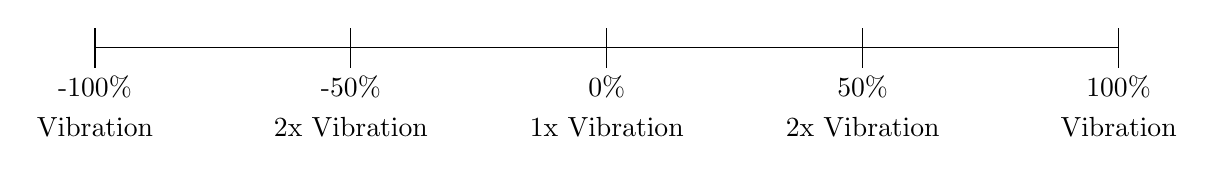
\begin{tikzpicture}
        \draw (0,0) -- (13,0);
        \draw (0,0.25) -- (0,-0.25);
        \draw (0,-0.5) node {-100\%};
        \draw (0,-1) node {Vibration};
        \draw (3.25, 0.25) -- (3.25, -0.25);
        \draw (3.25,-0.5) node {-50\%};
        \draw (3.25,-1) node {2x Vibration};
        \draw (6.5,0.25) -- (6.5,-0.25);
        \draw (6.5,-0.5) node {0\%};
        \draw (6.5,-1) node {1x Vibration};
        \draw (9.75,0.25) -- (9.75,-0.25);
        \draw (9.75,-0.5) node {50\%};
        \draw (9.75,-1) node {2x Vibration};
        \draw (13,0.25) -- (13,-0.25);
        \draw (13,-0.5) node {100\%};
        \draw (13,-1) node {Vibration};
    \end{tikzpicture}
\end{figure}
\\
Dabei ist die Schwelle so gewählt, dass die Vibrationen nicht zu oft ausgelöst werden. 
Es ist wichtig zu wissen, dass der Wert basierend auf der Eingabe des Joysticks kontinuierlich berechnet wird.
Die Eingabe beträgt -1 bis 1. Dabei ist -1 die maximale Position nach links und 1 die maximale Position nach rechts.
Damit die Ruderstellung nicht zu schnell verändert wird, benötigt diese eine volle Eingabe von 1 oder -1 für 2 Sekunden,
damit die Ruderstellung 100\% erreicht. Entsprechend werden die 100\% langsamer erreicht, wenn die Eingabe geringer
ist.
